\documentclass[conference]{IEEEtran}

\usepackage{cite}
\usepackage{amsmath,amssymb,amsfonts}
\usepackage{algorithmic}
\usepackage{graphicx}
\usepackage{textcomp}
\usepackage{xcolor}
\usepackage{booktabs}
\usepackage{multirow}
\usepackage{array}
\usepackage{url}
\usepackage{hyperref}
\usepackage{tikz}
\usetikzlibrary{shapes,arrows,positioning,fit,backgrounds}

\hypersetup{colorlinks=true,linkcolor=blue,urlcolor=blue,citecolor=blue}

\def\BibTeX{{\rm B\kern-.05em{\sc i\kern-.025em b}\kern-.08em
    T\kern-.1667em\lower.7ex\hbox{E}\kern-.125emX}}

\begin{document}

\title{Deep Learning-Based Disease Detection in Arecanut Using MobileNetV2}

\author{
\IEEEauthorblockN{Athmika Shetty}
\IEEEauthorblockA{Department of Master of Computer Applications\\
NMAM Institute of Technology\\
Nitte, Karnataka, India}
\and
\IEEEauthorblockN{[Second Author's Full Name]}
\IEEEauthorblockA{Department of Master of Computer Applications\\
NMAM Institute of Technology\\
Nitte, Karnataka, India}
}

\maketitle

\begin{abstract}
Arecanut (\textit{Areca catechu} L.) cultivation in India is affected by multiple diseases that reduce yield and quality if not identified early. This paper presents an image-based disease classification system for arecanut plants using MobileNetV2 transfer learning. A convolutional neural network based on the MobileNetV2 architecture, pretrained on ImageNet, is fine-tuned to classify arecanut images into nine categories: four healthy conditions (Healthy\_Leaf, Healthy\_Nut, Healthy\_Trunk, healthy\_foot) and five disease conditions (Mahali\_Koleroga, Stem\_bleeding, bud borer, stem cracking, yellow leaf disease). The model was trained on 8{,}514 images, validated on 1{,}835 images, and evaluated on 1{,}943 test images using a source-group stratified split to mitigate data leakage from augmented images. On the offline test set, the model achieved 96.76\% accuracy, a macro F1-score of 93.55\%, and a weighted F1-score of 96.80\%. The trained model is integrated into a web application built with React and Flask, enabling users to upload arecanut photographs and receive a predicted class with a model confidence score. We discuss class imbalance, limited source-image diversity, and a preprocessing discrepancy between the evaluation and application pipelines as threats to validity that must be addressed before deployment.
\end{abstract}

\begin{IEEEkeywords}
arecanut disease detection, deep learning, MobileNetV2, transfer learning, image classification, plant pathology, convolutional neural networks
\end{IEEEkeywords}

% ======================================================================
\section{Introduction}
% ======================================================================

Arecanut (\textit{Areca catechu} L.) is a major commercial crop cultivated across the coastal and Malnad regions of Karnataka, Kerala, and other Indian states. India is the largest producer of arecanut, with an annual production exceeding 800{,}000 tonnes \cite{arecanut_production}. The crop is vulnerable to several diseases and physiological disorders, including Mahali or Koleroga (\textit{Phytophthora arecae}), stem bleeding disease (\textit{Ceratocystis paradoxa}), bud borer infestation, stem cracking, and yellow leaf disease. Early identification of these conditions is essential for timely intervention and yield protection.

Traditional disease identification relies on visual inspection by agricultural extension officers or experienced farmers. This approach is labor-intensive, subjective, and constrained by the availability of trained personnel, especially in rural areas. Deep learning-based image classification offers a complementary approach: a model trained on labelled disease images can provide rapid, automated predictions from photographs captured with a standard camera or smartphone.

Convolutional neural networks (CNNs) have demonstrated strong performance in plant disease detection across multiple crops. Mohanty \textit{et al.}~\cite{mohanty2016} trained a CNN on over 54{,}000 leaf images spanning 14 crop species and 26 diseases, achieving 99.35\% accuracy on held-out images. Ferentinos \cite{ferentinos2018} used VGG-based architectures on a similar plant disease dataset, reporting accuracy above 99\%. However, these studies note a significant drop in performance when models are tested on images collected under conditions different from training~\cite{mohanty2016}, underscoring the challenge of generalisation.

MobileNetV2~\cite{sandler2018} is a lightweight CNN architecture designed for mobile and resource-constrained environments. Its inverted residual structure with linear bottlenecks enables efficient inference while maintaining competitive accuracy, making it suitable for agricultural applications where computational resources may be limited.

This paper presents a complete system for arecanut disease classification using MobileNetV2 transfer learning. The contributions of this work are:
\begin{enumerate}
    \item A nine-class arecanut health and disease classification model based on MobileNetV2 with a custom classification head, trained using a two-phase transfer learning strategy.
    \item A source-group stratified data split that mitigates leakage from augmented images sharing the same original photograph.
    \item A web application integrating the trained model with a React frontend and Flask backend, enabling image upload and real-time prediction.
    \item An honest evaluation that reports not only aggregate metrics but also per-class limitations, class imbalance effects, and a preprocessing discrepancy between the offline evaluation and live application pipelines.
\end{enumerate}

% ======================================================================
\section{Related Work}
\label{sec:related}
% ======================================================================

\subsection{Deep Learning for Plant Disease Detection}

The application of CNNs to plant disease detection has grown rapidly since 2016. Mohanty \textit{et al.}~\cite{mohanty2016} used the AlexNet and GoogLeNet architectures on the PlantVillage dataset, demonstrating that deep learning can automatically identify crop diseases from leaf images with high accuracy. However, their model's accuracy dropped to 31.4\% when tested on images collected from the web under uncontrolled conditions, highlighting the generalisation challenge.

Ferentinos \cite{ferentinos2018} trained multiple CNN architectures, including VGG and CNN models inspired by AlexNet, on 87{,}848 images covering 25 plant species and 61 disease classes. The best model achieved 99.53\% accuracy, but the study relied on images captured under controlled laboratory conditions with uniform backgrounds.

A common limitation across these studies is the use of datasets with images collected under controlled conditions (uniform backgrounds, consistent lighting). Real-world field images introduce variability in background, illumination, and viewing angle, which can significantly degrade model performance~\cite{mohanty2016}.

\subsection{Transfer Learning and MobileNetV2}

Transfer learning~\cite{pan2010} leverages knowledge learned on a source task to improve performance on a target task. In image classification, CNN architectures pretrained on the ImageNet dataset~\cite{russakovsky2015} serve as feature extractors for domain-specific tasks. The early layers of a CNN learn general visual features (edges, textures, colour gradients) that transfer well across domains, while later layers capture task-specific patterns.

MobileNetV2~\cite{sandler2018} introduces the inverted residual block with linear bottlenecks. Unlike traditional residual blocks that connect wide layers, MobileNetV2 connects thin bottleneck layers via shortcut connections. The intermediate expansion layer uses lightweight depthwise separable convolutions~\cite{howard2017} to filter features. This design reduces the number of parameters and computational operations while preserving representational capacity.

MobileNetV2 has been applied to plant disease detection in several studies, where its computational efficiency makes it suitable for deployment on mobile devices or edge servers in agricultural settings. The pretrained ImageNet weights provide a strong initialization for visual feature extraction, reducing the amount of domain-specific training data required.

\subsection{Research Gap}

While deep learning has been extensively applied to disease detection in crops such as tomato, maize, and grape, its application to arecanut specifically has received limited attention. Arecanut diseases present unique visual characteristics---stem-based symptoms (stem bleeding, stem cracking), nut-level conditions, and canopy-level yellowing---that differ from the leaf-focused symptoms common in other crop disease datasets. The available arecanut image datasets are relatively small and often heavily augmented, raising concerns about data leakage and generalisation. This work addresses these gaps by applying MobileNetV2 transfer learning to a nine-class arecanut classification task with a source-group stratified split and an integrated web application.

% ======================================================================
\section{Dataset Description}
\label{sec:dataset}
% ======================================================================

The dataset used in this study contains 12{,}292 images across nine arecanut health and disease categories. The images were organised using a leakage-free source-group stratified split, as described in Section~\ref{sec:methodology}. Table~\ref{tab:dataset} summarises the partition sizes.

\begin{table}[htbp]
\caption{Dataset partition sizes}
\label{tab:dataset}
\centering
\begin{tabular}{l|r}
\toprule
\textbf{Partition} & \textbf{Image files} \\
\midrule
Training       & 8{,}514 \\
Validation     & 1{,}835 \\
Testing        & 1{,}943 \\
\midrule
\textbf{Total} & \textbf{12{,}292} \\
\bottomrule
\end{tabular}
\end{table}

A critical characteristic of this dataset is that the 12{,}292 image files do \emph{not} represent 12{,}292 independently collected field photographs. The images are augmented or derived copies of approximately 1{,}226 original source images. Each source image was used to generate multiple augmented variants through geometric and photometric transformations. Consequently, the effective diversity of the dataset is determined by the number of independent source photographs, not the total file count.

This distinction has two important implications:
\begin{enumerate}
    \item \textbf{Data leakage risk:} If augmented copies of the same source image are split across training and test partitions, the test accuracy may be inflated because the model has effectively seen variations of the same visual content during training. The source-group stratified split (Section~\ref{sec:methodology}) addresses this by ensuring that all augmented copies of a given source image remain in one partition.
    \item \textbf{Generalisation limitation:} Even with leakage-free splitting, the model's performance on these 1{,}943 test images does not guarantee similar performance on independently collected field images from different locations, seasons, or camera devices.
\end{enumerate}

The nine classes and their approximate source-group counts are listed in Table~\ref{tab:classes}. The dataset exhibits significant class imbalance: the largest class (Mahali\_Koleroga) contains approximately 3{,}560 images derived from 356 source groups, while the smallest class (healthy\_foot) contains only 70 images derived from 7 source groups---a ratio of approximately 51:1.

\begin{table}[htbp]
\caption{Class distribution across all partitions}
\label{tab:classes}
\centering
\small
\begin{tabular}{l|r|r|r|r}
\toprule
\textbf{Class} & \textbf{Train} & \textbf{Val} & \textbf{Test} & \textbf{Total} \\
\midrule
Healthy\_Leaf        & 583 & 133 & 124 & 840 \\
Healthy\_Nut          & 1{,}845 & 383 & 392 & 2{,}620 \\
Healthy\_Trunk        & 1{,}363 & 290 & 337 & 1{,}990 \\
Mahali\_Koleroga      & 2{,}458 & 546 & 556 & 3{,}560 \\
Stem\_bleeding        & 151 & 28 & 31 & 210 \\
bud borer             & 141 & 28 & 31 & 200 \\
healthy\_foot         & 48 & 11 & 11 & 70 \\
stem cracking         & 513 & 102 & 135 & 750 \\
yellow leaf disease   & 1{,}412 & 314 & 326 & 2{,}052 \\
\midrule
\textbf{Total}        & \textbf{8{,}514} & \textbf{1{,}835} & \textbf{1{,}943} & \textbf{12{,}292} \\
\bottomrule
\end{tabular}
\end{table}

% ======================================================================
\section{Proposed Methodology}
\label{sec:methodology}
% ======================================================================

\subsection{Source-Group Stratified Split}

To prevent data leakage from augmented images sharing the same original source photograph, a source-group stratified split was employed. The filename of each image encodes its source identity in the pattern \texttt{<class>\_original\_<source\_id>\_<UUID>.jpg}, where \texttt{source\_id} identifies the original photograph and \texttt{UUID} is a unique identifier for each augmented copy.

The split operates at the source-group level: all augmented copies of a given source image are assigned to exactly one of the three partitions (train, validation, or test). The split ratio is 70\% training, 15\% validation, and 15\% testing, applied independently per class to maintain class proportions across partitions. A fixed random seed (42) ensures reproducibility.

This approach prevents the most direct form of data leakage---where pixel-similar augmented copies of the same source appear in both training and test sets. However, it does not eliminate all forms of similarity: different source images captured during the same field session may share visual characteristics (lighting, background, camera angle) that the model can exploit.

\subsection{Model Architecture}

The classification model uses MobileNetV2~\cite{sandler2018} as the backbone architecture with ImageNet~\cite{russakovsky2015} pretrained weights. The pretrained MobileNetV2 base (excluding the top classification layer) produces feature maps of shape $7 \times 7 \times 1280$ from $224 \times 224 \times 3$ input images. A custom classification head is added:

\begin{enumerate}
    \item \textbf{Global Average Pooling 2D:} Reduces each feature map to a single value, producing a 1280-dimensional vector.
    \item \textbf{Dense layer (128 units, ReLU):} A fully connected layer with 128 neurons and rectified linear unit activation~\cite{nair2010} for non-linear feature combination.
    \item \textbf{Dropout (rate = 0.3):} Randomly deactivates 30\% of neurons during training to mitigate overfitting~\cite{srivastava2014}.
    \item \textbf{Dense layer (9 units, softmax):} The final classification layer with softmax activation, producing a probability distribution over the nine classes.
\end{enumerate}

The total model has 2{,}423{,}113 parameters, of which 165{,}129 are trainable during the first training phase (the classification head only). The MobileNetV2 backbone contributes 2{,}257{,}984 parameters, which are initially frozen.

\subsection{Training Procedure}

Training proceeds in two phases, following a standard transfer learning strategy~\cite{pan2010}:

\textbf{Phase 1 --- Frozen backbone (20 epochs):} The MobileNetV2 backbone is frozen, and only the custom classification head is trained. The learning rate is set to $10^{-3}$ using the Adam optimiser~\cite{kingma2015}. This phase allows the randomly initialised classification head to learn task-specific weights while leveraging the pretrained features from the backbone.

\textbf{Phase 2 --- Fine-tuning (up to 10 epochs):} The top 30 layers of the MobileNetV2 backbone are unfrozen for fine-tuning. The learning rate is reduced to $10^{-4}$ to prevent large weight updates that could destroy the pretrained features. Early stopping with a patience of 5 epochs on validation accuracy terminates training when no improvement is observed.

Additional training configuration:
\begin{itemize}
    \item \textbf{Batch size:} 32
    \item \textbf{Loss function:} Sparse categorical cross-entropy
    \item \textbf{Class weights:} Computed using the balanced strategy to counteract class imbalance. Classes with fewer samples receive higher weights (e.g., healthy\_foot weight $\approx$ 19.7, Mahali\_Koleroga weight $\approx$ 0.38).
    \item \textbf{Data augmentation:} Random horizontal flip, random brightness ($\pm 0.1$), and random contrast ($0.9$--$1.1$) applied to training images.
    \item \textbf{Callbacks:} Early stopping (monitor validation accuracy, patience = 5, restore best weights), ReduceLROnPlateau (monitor validation loss, factor = 0.5, patience = 3), and ModelCheckpoint (save best model on validation accuracy).
    \item \textbf{Random seed:} 42 (fixed for reproducibility).
\end{itemize}

Phase 1 completed all 20 epochs, reaching a best validation accuracy of 93.30\%. Phase 2 was early-stopped after 7 epochs, reaching a best validation accuracy of 95.42\%.

\subsection{Image Preprocessing}

The training and evaluation pipeline preprocesses each image as follows:
\begin{enumerate}
    \item Decode the JPEG image to a tensor using TensorFlow's \texttt{tf.image.decode\_jpeg}.
    \item Resize to $224 \times 224$ pixels using TensorFlow's \texttt{tf.image.resize}.
    \item Apply MobileNetV2 preprocessing: \texttt{tf.keras.applications.mobilenet\_v2.preprocess\_input}, which scales pixel values from $[0, 255]$ to $[-1, 1]$.
    \item Add a batch dimension to produce a tensor of shape $(1, 224, 224, 3)$.
\end{enumerate}

\textit{Preprocessing discrepancy:} The web application uses Pillow (Python Imaging Library) for image decoding and resizing instead of TensorFlow's image operations. While both libraries implement bilinear interpolation, their implementations differ in detail (antialiasing, boundary handling, colour space conversion). This discrepancy can cause subtle differences in the preprocessed pixel values for the same input image, potentially leading to different predictions between the evaluation pipeline and the live application. This limitation is discussed further in Section~\ref{sec:limitations}.

% ======================================================================
\section{System Architecture}
\label{sec:system}
% ======================================================================

The complete system consists of a React frontend, a Flask backend, and the trained MobileNetV2 model. Figure~\ref{fig:architecture} shows the overall architecture.

\begin{figure}[htbp]
\centering
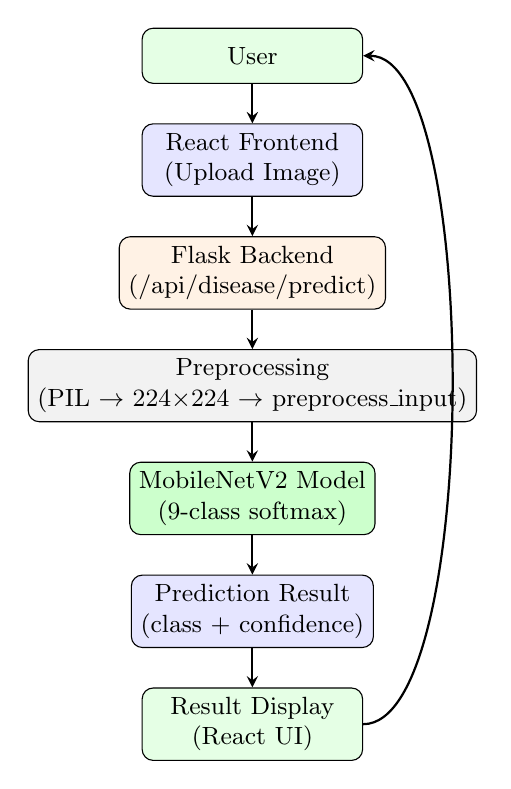
\begin{tikzpicture}[
    node distance=0.5cm,
    box/.style={draw, rounded corners, minimum width=2.8cm, minimum height=0.7cm, align=center, font=\small},
    arrow/.style={->, thick, >=stealth}
]
\node[box, fill=green!10] (user) {User};
\node[box, fill=blue!10, below=of user] (frontend) {React Frontend\\(Upload Image)};
\node[box, fill=orange!10, below=of frontend] (backend) {Flask Backend\\(/api/disease/predict)};
\node[box, fill=gray!10, below=of backend] (preprocess) {Preprocessing\\(PIL $\to$ 224$\times$224 $\to$ preprocess\_input)};
\node[box, fill=green!20, below=of preprocess] (model) {MobileNetV2 Model\\(9-class softmax)};
\node[box, fill=blue!10, below=of model] (result) {Prediction Result\\(class + confidence)};
\node[box, fill=green!10, below=of result] (display) {Result Display\\(React UI)};

\draw[arrow] (user) -- (frontend);
\draw[arrow] (frontend) -- (backend);
\draw[arrow] (backend) -- (preprocess);
\draw[arrow] (preprocess) -- (model);
\draw[arrow] (model) -- (result);
\draw[arrow] (result) -- (display);
\draw[arrow] (display.east) .. controls +(1.5,0) and +(1.5,0) .. (user.east);
\end{tikzpicture}
\caption{Overall system architecture. The user uploads an image through the React frontend, which sends it to the Flask backend. The backend preprocesses the image, runs the MobileNetV2 model, and returns the predicted class and confidence score.}
\label{fig:architecture}
\end{figure}

\subsection{Frontend}

The frontend is built with React 18 using the Create React App framework. The disease detection page provides:
\begin{itemize}
    \item A drag-and-drop upload area accepting JPG, PNG, and WEBP images (maximum 16 MB).
    \item Client-side file type and size validation before uploading.
    \item An image preview with a remove button.
    \item An ``Analyse for Disease'' button that sends the image to the backend via a \texttt{POST} request with \texttt{FormData}.
    \item Loading state with a disabled button and ``Analysing\ldots'' text during the API call.
    \item Error display if the backend is unreachable or returns an error.
    \item A result card showing the predicted class name, a status badge (green for healthy, red for disease), a confidence bar, and all nine class scores with progress bars.
    \item A disclaimer stating that the confidence is a raw softmax score, not a calibrated probability, and that the result should not replace expert diagnosis.
\end{itemize}

The frontend uses a proxy configuration (\texttt{"proxy": "http://localhost:5000"}) so that API calls to \texttt{/api/disease/predict} are forwarded to the Flask backend during development.

\subsection{Backend}

The backend is built with Flask 3.0.3 and uses flask-cors for cross-origin resource sharing. The trained model and class mapping are loaded once at application startup via a \texttt{load\_disease\_model()} function, storing the model in module-level variables that persist across requests. This avoids the overhead of loading the 22.74\,MB model on every request.

The prediction endpoint (\texttt{POST /api/disease/predict}) accepts multipart form data with the image file under the key \texttt{image}. The processing pipeline is:
\begin{enumerate}
    \item Validate file presence, extension (JPG, JPEG, PNG, WEBP), and size ($\leq$ 16\,MB).
    \item Read file bytes and decode the image using Pillow's \texttt{Image.open}.
    \item Convert to RGB, resize to $224 \times 224$ using bilinear interpolation.
    \item Apply \texttt{mobilenet\_v2.preprocess\_input} to scale pixel values to $[-1, 1]$.
    \item Run model inference: \texttt{model.predict()} produces a 9-element softmax vector.
    \item Map the highest-scoring index to a class name using \texttt{class\_indices.json}.
    \item Return a JSON response with the predicted class, confidence score, all class scores, and the calibration disclaimer.
\end{enumerate}

A health endpoint (\texttt{GET /api/health}) returns the server status and whether the model loaded successfully.

% ======================================================================
\section{Experimental Setup}
\label{sec:setup}
% ======================================================================

\subsection{Training Environment}

Training was performed on a Windows machine with TensorFlow 2.21.0 using CPU only (GPU support is not available on native Windows for TensorFlow $\geq$ 2.11). Python 3.12.3 was used with NumPy 2.5.2 and Pillow 12.3.0.

\subsection{Evaluation Metrics}

The model is evaluated on the 1{,}943-image test partition using the following metrics:

\textbf{Accuracy:}
\begin{equation}
\text{Accuracy} = \frac{TP + TN}{TP + TN + FP + FN}
\end{equation}

\textbf{Precision (per class):}
\begin{equation}
\text{Precision}_c = \frac{TP_c}{TP_c + FP_c}
\end{equation}

\textbf{Recall (per class):}
\begin{equation}
\text{Recall}_c = \frac{TP_c}{TP_c + FN_c}
\end{equation}

\textbf{F1-score (per class):}
\begin{equation}
F1_c = 2 \cdot \frac{\text{Precision}_c \cdot \text{Recall}_c}{\text{Precision}_c + \text{Recall}_c}
\end{equation}

\textbf{Macro averages} are computed as the unweighted mean of per-class precision, recall, and F1-score, giving equal weight to each class regardless of support. \textbf{Weighted averages} are computed as the support-weighted mean, giving more influence to classes with more test samples.

% ======================================================================
\section{Experimental Results}
\label{sec:results}
% ======================================================================

\subsection{Overall Performance}

Table~\ref{tab:overall} presents the overall evaluation metrics on the 1{,}943-image test partition.

\begin{table}[htbp]
\caption{Overall test set evaluation metrics}
\label{tab:overall}
\centering
\begin{tabular}{l|r}
\toprule
\textbf{Metric} & \textbf{Result} \\
\midrule
Accuracy              & 96.76\% \\
Macro precision       & 92.91\% \\
Macro recall          & 94.56\% \\
Macro F1-score        & 93.55\% \\
Weighted precision    & 96.96\% \\
Weighted recall       & 96.76\% \\
Weighted F1-score     & 96.80\% \\
\bottomrule
\end{tabular}
\end{table}

The model achieves 96.76\% accuracy on the test set. The macro F1-score (93.55\%) is lower than the weighted F1-score (96.80\%) because macro averaging gives equal weight to small classes (Stem\_bleeding: support = 31, healthy\_foot: support = 11), which have lower per-class F1-scores.

\subsection{Class-wise Performance}

Table~\ref{tab:perclass} presents the per-class precision, recall, F1-score, and support from the test set evaluation.

\begin{table*}[htbp]
\caption{Per-class evaluation results on the 1{,}943-image test partition}
\label{tab:perclass}
\centering
\small
\begin{tabular}{l|r|r|r|r}
\toprule
\textbf{Class} & \textbf{Precision} & \textbf{Recall} & \textbf{F1-score} & \textbf{Support} \\
\midrule
Healthy\_Leaf        & 1.0000 & 0.9677 & 0.9836 & 124 \\
Healthy\_Nut         & 0.9948 & 0.9796 & 0.9871 & 392 \\
Healthy\_Trunk       & 0.9969 & 0.9555 & 0.9758 & 337 \\
Mahali\_Koleroga     & 0.9858 & 0.9964 & 0.9911 & 556 \\
Stem\_bleeding       & 0.8158 & 1.0000 & 0.8986 & 31 \\
bud borer            & 0.8750 & 0.9032 & 0.8889 & 31 \\
healthy\_foot        & 0.9000 & 0.8182 & 0.8571 & 11 \\
stem cracking        & 0.8442 & 0.9630 & 0.8997 & 135 \\
yellow leaf disease  & 0.9497 & 0.9264 & 0.9379 & 326 \\
\midrule
\textbf{Macro avg}   & \textbf{0.9291} & \textbf{0.9456} & \textbf{0.9355} & \textbf{1{,}943} \\
\textbf{Weighted avg}& \textbf{0.9696} & \textbf{0.9676} & \textbf{0.9680} & \textbf{1{,}943} \\
\bottomrule
\end{tabular}
\end{table*}

The four healthy classes and Mahali\_Koleroga achieve F1-scores above 0.97, indicating strong classification performance. The disease classes with limited test support show lower F1-scores:
\begin{itemize}
    \item \textbf{Stem\_bleeding} (F1 = 0.8986, support = 31): While recall is 1.0000 (all true Stem\_bleeding images are correctly identified), precision is 0.8158, meaning some images from other classes are misclassified as Stem\_bleeding. This suggests visual similarity between Stem\_bleeding and other classes.
    \item \textbf{healthy\_foot} (F1 = 0.8571, support = 11): With only 11 test images derived from 1 source group, this class has the least statistical reliability. The recall of 0.8182 means 2 of 11 images are misclassified.
    \item \textbf{bud borer} (F1 = 0.8889, support = 31): Both precision and recall are below 0.91, indicating bidirectional confusion with other classes.
    \item \textbf{stem cracking} (F1 = 0.8997, support = 135): Recall is strong at 0.9630 but precision is 0.8442, meaning some non-stem-cracking images are predicted as this class.
\end{itemize}

\subsection{Confusion Matrix}

Figure~\ref{fig:confusion} shows the normalised confusion matrix from the test set evaluation. The diagonal elements represent the proportion of correctly classified images per class.

\begin{figure}[htbp]
\centering
% PLACEHOLDER: Replace with actual confusion_matrix.png
% File location: ml/disease/results/confusion_matrix.png
% Upload to Overleaf as confusion_matrix.png
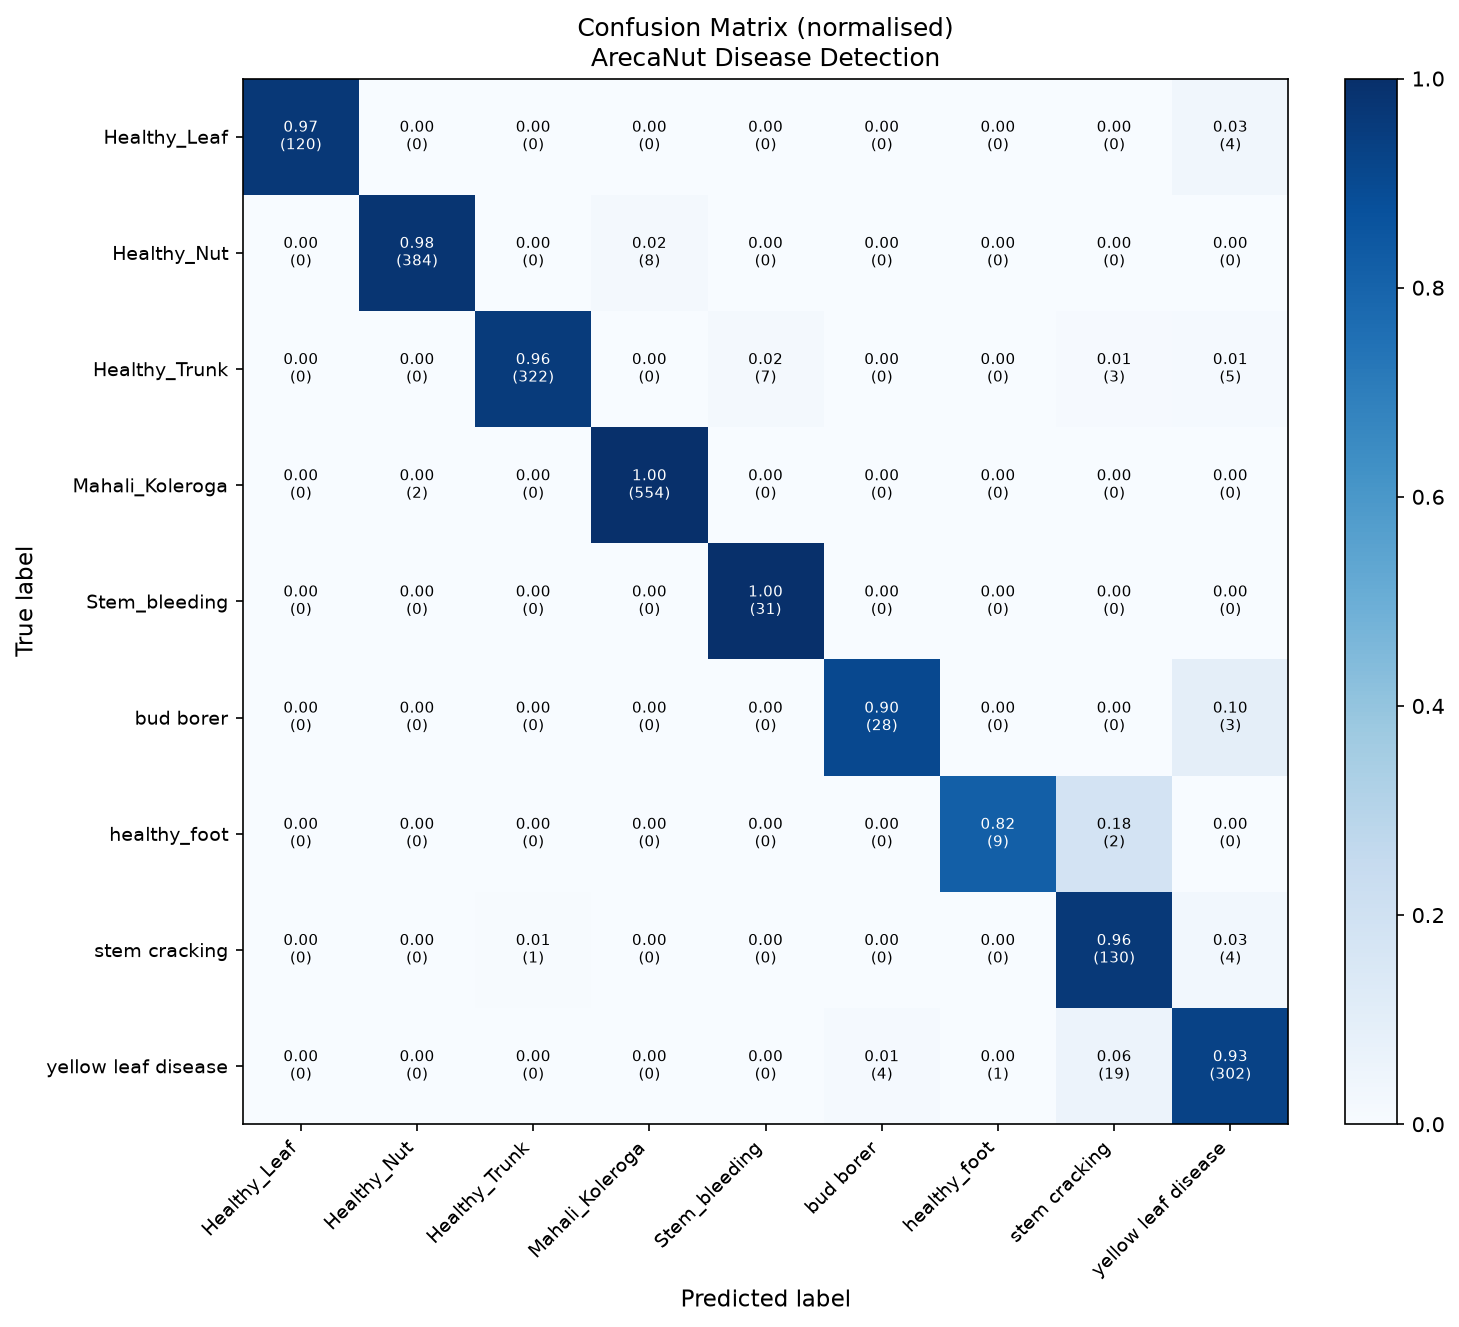
\includegraphics[width=\columnwidth]{confusion_matrix.png}
\caption{Normalised confusion matrix for the nine-class arecanut disease classifier on the 1{,}943-image test set. Diagonal values represent per-class recall. Off-diagonal values indicate misclassification rates.}
\label{fig:confusion}
\end{figure}

The confusion matrix confirms that the dominant confusion patterns occur among classes with limited training data and visual similarity. Healthy\_Trunk images are occasionally confused with other healthy classes, and Stem\_bleeding is sometimes confused with yellow leaf disease, consistent with the precision-recall trade-off observed in Table~\ref{tab:perclass}.

\subsection{Training Curves}

Figure~\ref{fig:training} shows the training and validation accuracy and loss across all 27 epochs (20 in Phase~1, 7 in Phase~2).

\begin{figure}[htbp]
\centering
% PLACEHOLDER: Replace with actual accuracy_loss_plot.png
% File location: ml/disease/results/accuracy_loss_plot.png
% Upload to Overleaf as accuracy_loss_plot.png
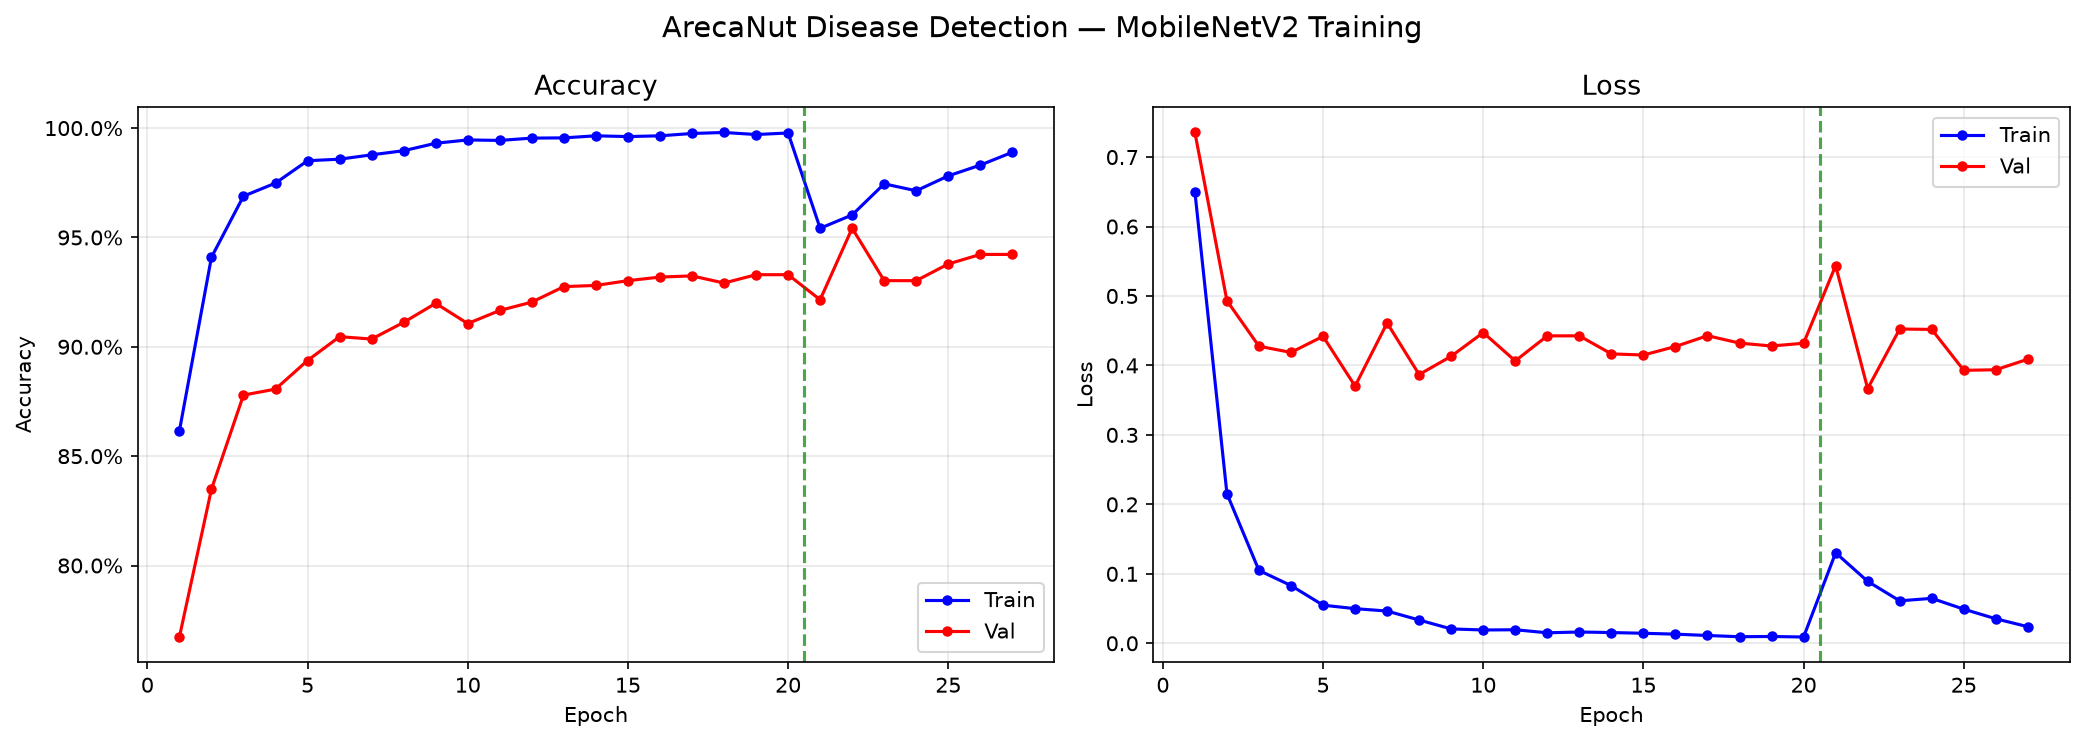
\includegraphics[width=\columnwidth]{accuracy_loss_plot.png}
\caption{Training and validation accuracy (top) and loss (bottom) over 27 epochs. The vertical dashed line marks the transition from Phase~1 (frozen backbone) to Phase~2 (fine-tuning). Phase~2 improves validation accuracy from 93.30\% to 95.42\%.}
\label{fig:training}
\end{figure}

During Phase~1, training accuracy rises rapidly to over 99\% within 10 epochs, while validation accuracy plateaus at approximately 93\%. This gap indicates some overfitting, which is expected given the limited source-image diversity. Phase~2 fine-tuning improves validation accuracy to 95.42\%, confirming that adapting the upper backbone layers to the arecanut domain provides a measurable benefit.

% ======================================================================
\section{Discussion}
\label{sec:discussion}
% ======================================================================

\subsection{Comparison with Related Research}

Table~\ref{tab:comparison} compares the proposed system with related plant disease detection studies. Direct comparison is limited because the datasets, crop types, and class structures differ substantially.

\begin{table}[htbp]
\caption{Comparison with related plant disease detection studies}
\label{tab:comparison}
\centering
\small
\begin{tabular}{p{1.5cm}p{1.5cm}p{1.2cm}p{1.5cm}}
\toprule
\textbf{Study} & \textbf{Crop} & \textbf{Classes} & \textbf{Reported accuracy} \\
\midrule
Mohanty \cite{mohanty2016} & 14 crops & 26 & 99.35\%$^*$ \\
Ferentinos \cite{ferentinos2018} & 25 plants & 61 & 99.53\%$^*$ \\
This work & Arecanut & 9 & 96.76\% \\
\bottomrule
\multicolumn{4}{l}{\scriptsize $^*$Tested on images from the same controlled dataset.}
\end{tabular}
\end{table}

The reported accuracy of 96.76\% is lower than the 99\%+ accuracy reported in \cite{mohanty2016} and \cite{ferentinos2018}. This difference is expected and does not imply inferior methodology. The studies in \cite{mohanty2016} and \cite{ferentinos2018} use the PlantVillage dataset, which contains images captured under controlled laboratory conditions with uniform backgrounds. The arecanut dataset used in this work contains field photographs with more visual variability. Additionally, both reference studies report significant accuracy drops when tested on images from different sources, confirming that high controlled-condition accuracy does not guarantee real-world performance.

\subsection{Effect of Class Imbalance}

The dataset has a class imbalance ratio of approximately 51:1 (Mahali\_Koleroga vs.\ healthy\_foot). Class weights were used during training to counteract this imbalance, giving underrepresented classes up to 19.7$\times$ more influence per sample. The effect is visible in the results: despite having only 11 test images, healthy\_foot achieves a recall of 0.8182, which would likely be near zero without class weighting.

However, class weighting cannot fully compensate for insufficient data diversity. The healthy\_foot class has only 7 independent source groups, meaning the model's representation of this class is based on very few unique visual examples. The precision--recall trade-off observed in Stem\_bleeding (perfect recall but low precision) suggests that the class weighting causes the model to be overly sensitive to this class, classifying similar-looking images from other classes as Stem\_bleeding.

% ======================================================================
\section{Limitations and Threats to Validity}
\label{sec:limitations}
% ======================================================================

Several limitations must be considered when interpreting the reported results.

\textbf{1. Augmented dataset, not independent field samples.} The 12{,}292 images are augmented copies of approximately 1{,}226 source photographs. The reported 96.76\% test accuracy reflects performance on augmented variations of these same 1{,}226 originals, not on independently collected field images. Performance on unseen real-world images from different locations, seasons, or camera devices has not been measured and may differ substantially. Mohanty \textit{et al.}~\cite{mohanty2016} observed a drop from 99.35\% to 31.4\% when testing on images from different sources, illustrating this risk.

\textbf{2. Preprocessing discrepancy.} The offline evaluation pipeline uses TensorFlow's \texttt{tf.image.decode\_jpeg} and \texttt{tf.image.resize} for image decoding and resizing, while the web application uses Pillow's \texttt{Image.open} and \texttt{Image.resize}. Although both use bilinear interpolation, their implementations differ in antialiasing, boundary handling, and internal colour space processing. A spot check confirmed that these differences can change the predicted class for the same input image. Consequently, the 96.76\% accuracy figure applies to the TensorFlow evaluation pipeline, not necessarily to the live web application. The application preprocessing must be aligned with the evaluation pipeline, and the complete application must be tested before deployment performance can be claimed.

\textbf{3. Limited source diversity for small classes.} The healthy\_foot class has only 7 source groups (11 test images), and Stem\_bleeding has 21 source groups (31 test images). Per-class metrics for these classes have low statistical reliability. A single misclassification changes the recall of healthy\_foot by 9 percentage points.

\textbf{4. No independent validation.} The model has not been tested on independently collected, correctly labelled field images. All evaluation is internal to the dataset.

\textbf{5. Confidence is not a calibrated probability.} The confidence score returned by the application is the raw softmax output for the predicted class. It is not a calibrated probability and should not be interpreted as the likelihood that the prediction is correct.

\textbf{6. Binary disease/healthy classification.} The frontend classifies predictions into ``disease detected'' (red) or ``no disease detected'' (green) based on the predicted class name. This binary grouping is a UI design choice and does not reflect a separate binary classifier. A misclassification at the nine-class level may also produce an incorrect binary status.

% ======================================================================
\section{Conclusion}
\label{sec:conclusion}
% ======================================================================

This paper presented a deep learning-based disease detection system for arecanut plants using MobileNetV2 transfer learning. The model classifies arecanut images into nine health and disease categories with 96.76\% test accuracy and a macro F1-score of 93.55\%. A source-group stratified split was employed to mitigate data leakage from augmented images, and class weighting addressed the significant class imbalance in the dataset.

The trained model was integrated into a web application with a React frontend and Flask backend, enabling users to upload arecanut photographs and receive a predicted disease class with a model confidence score. The system includes appropriate disclaimers about the nature of the confidence score and the need for expert verification.

The results demonstrate the feasibility of using lightweight pretrained CNN architectures for arecanut disease classification. However, the reported accuracy applies to an internal test set consisting of augmented images, and the preprocessing discrepancy between the evaluation and application pipelines must be resolved before the live application's performance can be claimed.

% ======================================================================
\section{Future Work}
\label{sec:future}
% ======================================================================

Several directions for future work are identified:
\begin{enumerate}
    \item \textbf{Align application preprocessing:} Replace Pillow-based preprocessing in the Flask backend with TensorFlow operations matching the evaluation pipeline, or re-evaluate the model using Pillow-based preprocessing, to eliminate the discrepancy.
    \item \textbf{Independent field validation:} Collect correctly labelled arecanut images from multiple field locations, seasons, and camera devices to measure real-world generalisation.
    \item \textbf{Expand small classes:} Collect additional source photographs for underrepresented classes (healthy\_foot, Stem\_bleeding, bud borer) to improve per-class reliability.
    \item \textbf{Calibration:} Apply temperature scaling or Platt scaling to the softmax outputs so that confidence scores are meaningful as calibrated probabilities.
    \item \textbf{Explainability:} Integrate Grad-CAM or similar techniques to visualise the image regions influencing each prediction, helping users understand and trust the model's output.
    \item \textbf{Comparison with other architectures:} Conduct a fair comparison with alternative lightweight architectures (e.g., EfficientNet, MobileNetV3) under identical dataset splits and training conditions.
\end{enumerate}

% ======================================================================
\section*{Acknowledgment}
% ======================================================================

The authors thank the Department of Master of Computer Applications, NMAM Institute of Technology, Nitte, for providing the computational resources and academic guidance for this project.

% ======================================================================
% References
% ======================================================================
\bibliographystyle{IEEEtran}

\begin{thebibliography}{99}

\bibitem{arecanut_production}
Ministry of Agriculture and Farmers Welfare, Government of India, ``Arecanut: Area, production, and yield statistics,'' \textit{Agricultural Statistics at a Glance}, 2023.

\bibitem{mohanty2016}
S.~P. Mohanty, D.~P. Hughes, and M.~Salath\'{e}, ``Using deep learning for image-based plant disease detection,'' \textit{Frontiers in Plant Science}, vol.~7, p.~1419, 2016.

\bibitem{ferentinos2018}
K.~P. Ferentinos, ``Deep learning models for plant disease detection and diagnosis,'' \textit{Computers and Electronics in Agriculture}, vol.~145, pp.~311--318, 2018.

\bibitem{sandler2018}
M.~Sandler, A.~Howard, M.~Zhu, A.~Zhmoginov, and L.-C. Chen, ``MobileNetV2: Inverted residuals and linear bottlenecks,'' in \textit{Proc. IEEE Conference on Computer Vision and Pattern Recognition (CVPR)}, 2018, pp.~4510--4520.

\bibitem{pan2010}
S.~J. Pan and Q.~Yang, ``A survey on transfer learning,'' \textit{IEEE Transactions on Knowledge and Data Engineering}, vol.~22, no.~10, pp.~1345--1359, 2010.

\bibitem{russakovsky2015}
O.~Russakovsky \textit{et al.}, ``ImageNet large scale visual recognition challenge,'' \textit{International Journal of Computer Vision}, vol.~115, no.~3, pp.~211--252, 2015.

\bibitem{howard2017}
A.~Howard, M.~Zhu, B.~Chen, D.~Kalenichenko, W.~Wang, T.~Weyand, M.~Andreetto, and H.~Adam, ``MobileNets: Efficient convolutional neural networks for mobile vision applications,'' \textit{arXiv preprint arXiv:1704.04861}, 2017.

\bibitem{kingma2015}
D.~P. Kingma and J.~Ba, ``Adam: A method for stochastic optimization,'' in \textit{Proc. International Conference on Learning Representations (ICLR)}, 2015.

\bibitem{srivastava2014}
N.~Srivastava, G.~Hinton, A.~Krizhevsky, I.~Sutskever, and R.~Salakhutdinov, ``Dropout: A simple way to prevent neural networks from overfitting,'' \textit{Journal of Machine Learning Research}, vol.~15, pp.~1929--1958, 2014.

\bibitem{nair2010}
V.~Nair and G.~E. Hinton, ``Rectified linear units improve restricted Boltzmann machines,'' in \textit{Proc. International Conference on Machine Learning (ICML)}, 2010, pp.~807--814.

\bibitem{he2016}
K.~He, X.~Zhang, S.~Ren, and J.~Sun, ``Deep residual learning for image recognition,'' in \textit{Proc. IEEE Conference on Computer Vision and Pattern Recognition (CVPR)}, 2016, pp.~770--778.

\bibitem{shorten2019}
C.~Shorten and T.~M. Khoshgoftaar, ``A survey on image data augmentation for deep learning,'' \textit{Journal of Big Data}, vol.~6, no.~1, p.~60, 2019.

\bibitem{chollet2017}
F.~Chollet, ``Xception: Deep learning with depthwise separable convolutions,'' in \textit{Proc. IEEE Conference on Computer Vision and Pattern Recognition (CVPR)}, 2017, pp.~1251--1258.

\bibitem{too2019}
E.~C. Too, L.~Yujian, S.~Njuki, and L.~Yingchun, ``A comparative study of fine-tuning deep learning models for plant disease identification,'' \textit{Computers and Electronics in Agriculture}, vol.~161, pp.~272--279, 2019.

\end{thebibliography}

\end{document}
